% !TEX encoding = UTF-8 Unicode

\documentclass[twocolumn,10pt,a4j]{jsarticle}
\usepackage{kougai}

\title{シミュレータ教材を搭載した電子教科書制作のためのガイドライン作成}
\author{1532xxx 工大 太郎  指導教員 須田 宇宙 准教授}
\date{}

\begin{document}

\maketitle

\section{はじめに}
1章には,背景・問題点・目的を順番に書く.
背景は,広く一般的な事柄を書いて,読む人に同意を抱かせつつ問題点につなぐ.
問題点では,「〜という問題点がある」などのように,「問題」または「問題点」と言う単語を用いて,目的につなぐ.
目的では,「そこで本研究では」から始めて,「〜を目的とする」で締める.
以下は過去の卒業研究最終審査用の梗概の抜粋である.

%背景

近年ではタブレット端末の普及に伴い,オフライン状態で利用できる電子書籍が注目を集めている.
また本学でも,学生に対してiPadを配布しているため,全員が電子書籍を利用できる環境にある.

一方,音響教育関係者に使われているWeb版のシミュレータ教材群\cite{suda2018}がある.
これらは,目視することができない現象を可視化することや,仮想的な実験を行うことで,理解を促すことができる教材である.
本研究室では,これまでにシミュレータ教材の開発と配布が行われてきた.
また,「開発・カスタマイズガイドライン」を公開し,開発者・教育者のノウハウの共有も行われてきた.

%問題点
Web版のシミュレータ教材は,オフライン状態で利用できないことが問題点として挙げられる.
そこで,シミュレータ教材を電子書籍に搭載することで,オフライン状態でも利用できると考えた.
しかし,搭載して動作させる上で,シミュレータ教材の機能が制限される場合がある.
さらにシミュレータ教材をそのまま搭載しても,レイアウトの関係から利用しづらいという問題がある.
この問題に対して,音響教育関係者がノウハウを共有し,お互いの開発したシミュレータ教材をカスタマイズして電子書籍化することが望ましいと考えている.

%目的
そこで本研究では,音響教育関係者が容易に電子教科書を制作できるよう,シミュレータ教材を搭載した電子教科書のサンプルの制作と,その開発ガイドラインを作成し公開することを目的とする.

\section{電子教科書について}
2章では,研究テーマとして取り上げた内容(この例では「電子教科書」についての研究だった)について説明する.
その他,数式を用いて理論を説明することも可能である.

シミュレータ教材を利用する際には,シミュレートを行っている現象そのものについての理解を促す必要がある.
そのためには,シミュレーションの解説や教材の操作方法などを確認しながら利用することが,より効果的であると考えた.
この考えに基づいて制作した電子教科書の一部を図\ref{fig:教科書}に示す.
左側には,シミュレータに関する前提知識や解説を記述した.
右側には教材の操作方法を記述し,それを確認しながらシミュレータ教材を利用することを可能とした.
%電子教科書にはシミュレータ教材を6つ搭載し,全体で30ページほどの教科書を制作した.

一方,電子書籍の標準的フォーマットであるePub形式の電子書籍を閲覧できるリーダは限られている上,動作が安定しないことがある.
その中で,iPadに標準搭載されePub形式を閲覧可能であるiBooksを,本研究で利用するリーダとした.
そのためシミュレータ教材を搭載後,機能の動作確認はiBooksで行った.
iBooksではグラフ描画やアニメーションは可能であるが,音源再生や音声入力は実行できないことを確認した.%(できる気がしてきた)

\begin{figure}[h]
\begin{center}
 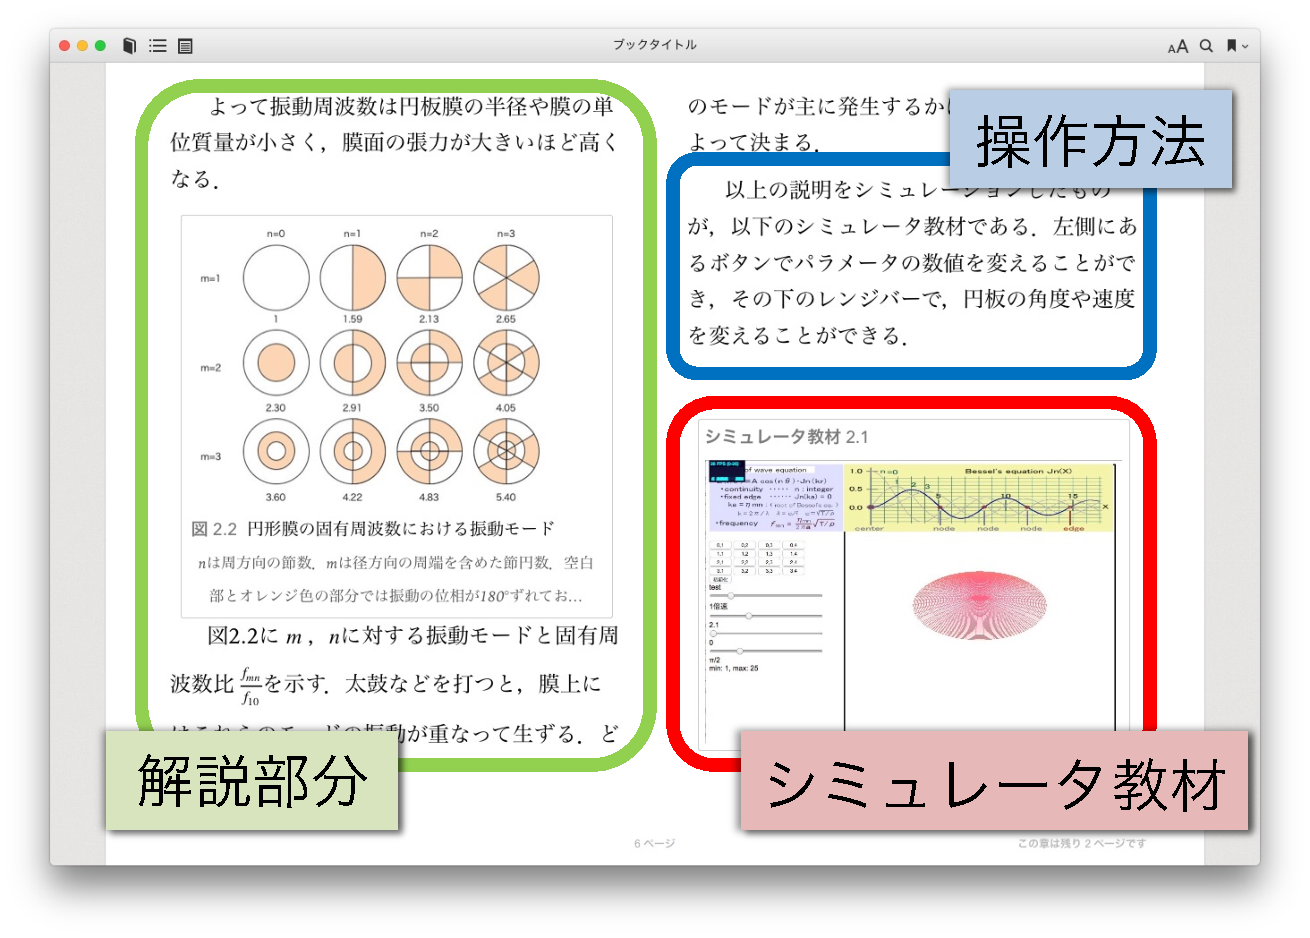
\includegraphics[clip,width=85mm,height=55mm]{textbook.pdf}
\end{center}
 \caption{電子教科書サンプル}
 \label{fig:教科書}
\end{figure}

\section{やること・やったこと}

3章には,中間審査用の梗概では実際に行う作業について(図を用いて)説明する.
最終審査用の梗概では,やったことを示す.
コンテンツを作成した場合にはコンテンツのスクリーンショットなどを用いる.
調査が主であれば,調査の概要と結果のグラフなどを使用する.

この文章では1章が長すぎるので,見た目のバランスが悪い.
通常の梗概の割合は左側に1章と2章,右側に3章と4章のように並ぶ.
もちろん多少の前後は有るので,きっちりと合わせなくても良い.

通常,図は2枚程度である.
図1枚+表1面でも構わない.
梗概を書き始める前に,使用する図を決めてからレイアウトしていくと雰囲気がつかみやすくて良い.




\section{今後の予定}
中間審査用の梗概では4章のタイトルとして「今後の予定」,最終審査用の梗概では「おわりに」などを用いる.
たいてい2〜3行程度でまとめる.

\begin{thebibliography}{99}
\bibitem{suda2018} 須田宇宙: ``音響科学e-Learning教材'', \url{https://www.sudalab.net/}, 2018/7/19参照
\end{thebibliography}

\end{document}